\begin{figure}[t]
  \centering
  %\includegraphics[width=\columnwidth]{figs/GOP_Goal.pdf}
  %\fbox{
  % left bottom right top
  %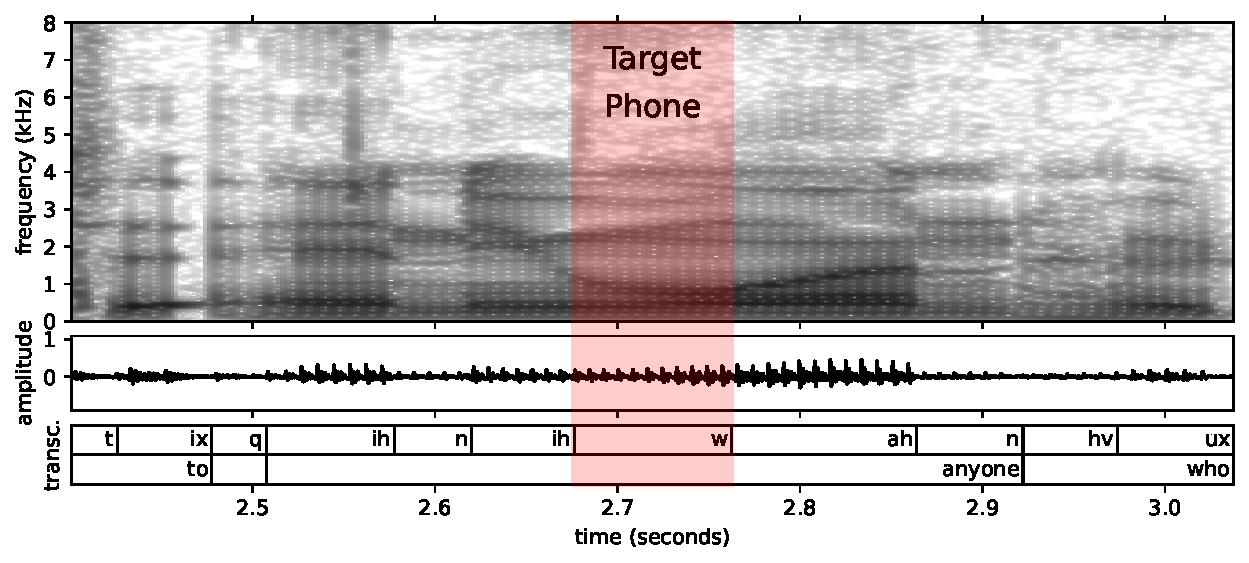
\includegraphics[width=\columnwidth, trim={65 0 70 30},clip]{figs/GOP_Goal2.pdf}
  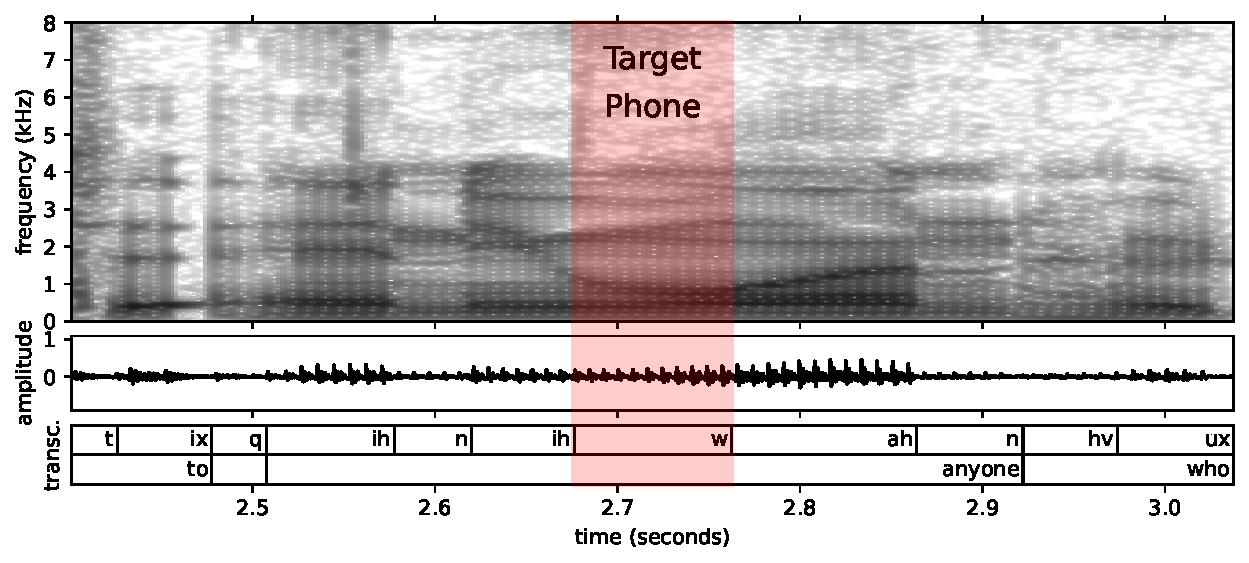
\includegraphics[width=\columnwidth]{figs/GOP_Goal2.pdf}
  %}
  \caption{Standard GOP methods use forced alignment to segment speech for analysis.}
  \label{fig:gop-goal}
\end{figure} 

\section{Background and Related Work}
\label{sec:Backgrounds}
In this section we give background information and review the related work that are necessary to understand the proposed method.
We will focus on phoneme-level pronunciation assessment that is the goal of this paper.
We first need to distinguish between continuous measures for pronunciation assessment and the specific task of MDD.
In the first case, the goal is to introduce a metric that can indicate how far a specific pronunciation of a phoneme is from the acceptable variability in the language.
An example of this kind of measure is GOP.
The MDD task, on the other hand, is to provide a binary or, sometimes ternary, decision on whether the pronunciation is correct or not.
This task can be performed 1) on a single GOP-like score by defining thresholds for the different output classes, 2) by more advanced classifiers based on multidimensional engineered features, or 3) by end-to-end systems that take raw speech as input.

In this paper, we focus on MDD methods that are based on GOP scores and GOP features.
We will first present the different definitions of GOP in Section~\ref{sec:gop_definitions},
the problem arising from the need for accurate speech segmentation in Section~\ref{sec:alignment_issues}, and, finally, the problem of using end-to-end peaky models with GOP in Section~\ref{sec:peaky_behavior}.

\subsection{The definition of GOP}
\label{sec:gop_definitions}
GOP was initially proposed as a measure of how closely the pronunciation of a specific phoneme matches its expected canonical pronunciation~\cite{witt2000phone}.
This is a segmental measure that requires time-aligned phonetic annotations (see, e.g., Figure~\ref{fig:gop-goal}).
Witt's original definition of GOP~\cite{witt2000phone} corresponds to the log posterior of the canonical phoneme $l_i$ given the sequence of observations $O_{t_1}^{t_2} = \{o_{t_1}, \dots, o_{t_2}\}$ in the segment under test, normalized by the sequence length:
\begin{equation}
    \label{eqa:gop}
    \text{GOP}(l_i)=\frac{\log(\mathit{p}(l_i|O_{t_1}^{t_2}))}{t_2-t_1}.
\end{equation}
Mispronunciations are detected on the basis of the GOP value and an empirically determined threshold. 

The estimation of the posteriors was originally implemented using Hidden Markov Models and Gaussian Mixture Models~(HMM-GMM) and by using Bayes rule:
\begin{equation}
    \label{eqa:gop2}
    \textit{p}(l_i|O_{t_1}^{t_2})=\frac{\mathit{p}(O_{t_1}^{t_2}|l_i)\mathit{P}(l_i)}{\sum_{q\in Q} \mathit{p}(O_{t_1}^{t_2}|q)\mathit{P}(q)},
\end{equation}
where $\mathit{P}(q)$ represents the prior probability of each phoneme in the phoneme inventory $Q$ and the likelihood $\mathit{p}(O_{t_1}^{t_2}|l_i)$ can be directly evaluated using the acoustic model, for example with the forward algorithm.
For efficiency reasons, Witt approximates the summation in the denominator by obtaining the best path over the full utterance through a phone-loop model.
From Eq.~\eqref{eqa:gop2}, GOP is then the ratio of the likelihood of the segment estimated from the canonical phone model (numerator) and the likelihood of the best path (allowing any phone sequence) through the segment (denominator). 

% either through manual transcriptions or forced alignment.
%With the conventional alignment-based GOP, the MDD usually works as follows:
%Firstly, the boundaries $t_1$ and $t_2$ of the target speech segment are
% corresponding to the target phoneme needs to be
%determined.
%The GOP value for the target phoneme is then computed using the features within the segment $O_{t_1}^{t_2} = \{o_{t_1}, \dots, o_{t_2}\}$ and with the help of an acoustic model trained for ASR.
The phoneme boundaries $t_1$ and $t_2$ could be obtained by human annotations.
However, this is not practical:
During model training, annotating large amounts of data would be too costly.
More importantly, this would make the methods not suitable for providing immediate and automated feedback to the students.
The segmentation step is, therefore, commonly automated by forced alignment using the canonical pronunciation  $\Lcano = \{l_1, \dots, l_{|\Lcano|}\}$ and a phonetic model trained for ASR.
This model does not need to be the same as that used for the GOP evaluation, and it is typically a context-independent HMM-GMM model.
%the given sequence of speech feature vectors $O_1^T = \{o_1, \dots, o_T\}$.
%This process is illustrated in Figure~\ref{fig:gop-goal}.


%The GOP can have various definitions. 
%The original definition from  is the log-posterior of the target phoneme $l_i$ normalized by the length of the segment $|t_2-t_1|$.
%Since the method is based on HMM-GMM models, we denote it as GOP-GMM:
%where $O_{t_1}^{t_2}$ represents the segment of the target phoneme $l_i$ obtained with an external aligner, which is usually a well-trained context-independent HMM-GMM model.
%since it is believed that a context-dependent model might not do the work well.
%The numerator is then divided.
%By using the Bayesian rule, the posterior in Eq.~\ref{eqa:gop} can be rewritten as:
%The division in Eq.~\eqref{eqa:gop2} is also considered as a normalization of irrelevant factors other than phoneme identities, for example, environmental noise, accent or other characteristics of different speakers.
%of
%Eq.~\eqref{eqa:gop2} are approximated by the Viterbi algorithm using the target phoneme with a single phoneme model .
%is often approximated by computing the probability of the frames within that segment according to the Viterbi path which is obtained by using a unconstrained phoneme-loop HMM structure.
%This leads to a trade-off between efficiency of calculation and performance
%approximation makes GOP more efficient without much loss of the performance
%\cite{witt-thesis}.
Although Witt's GOP has been successful, many later works argue that the phone-loop approximation is not reliable in estimating the denominator of Eq.~\ref{eqa:gop2}.
For example, Lattice-based GOP~\cite{Song2010LatticebasedGI} includes contributions from N-best hypotheses to avoid underestimating the value of the denominator.
%This helps because the lattice might store more optional paths that have locally higher probabilities than the sub-path of a globally maximum~(Viterbi) for estimating the GOP for the current phoneme.
In~\cite{luo2009analysis}, the authors show performance improvements that can be obtained when the phone-loop is evaluated multiple times over the target segment for each phoneme  rather than once along the whole utterance.
This implementation follows more closely the original definition of the denominator in Eq.\ref{eqa:gop2}.
%by using the proposed Forced-aligned GOP. 
%It forces to calculate the denominator of GOP within the alignment's segmentation separately for each phoneme. 

Phonological rules from the learner's first language~(L1) can also be included in the GOP methods, where the acoustic models are trained with target language~(L2) only, to achieve better accuracy~\cite{ERN, DUDY201862}.

The models used for estimating the GOP values are trained for ASR and therefore do not need any data that are annotated specifically for the MDD task.
However, in order to detect mispronunciations, 
%Even though GOP scores can be obtained without any human-annotated MDD data, it is often required to use 
a small amount of human-annotated data is required to estimate the optimal threshold that separates good pronunciations from bad ones.
These thresholds are usually phoneme-dependent but even finer-grained definitions (for example speaker-dependent) may improve accuracy (e.g. \cite{kanters09_slate}).
%In~\cite{kanters09_slate}, the authors show improved accuracy by defining speaker and phoneme dependent thresholds.
%the performance of GOP is studied in detail and they find that the optimization for the threshold operated on a fine-grained level~(the speakers) could improve the accuracy of MDD. 

Using hybrid HMM-Deep Neural Networks~(DNN) acoustic models has been shown to improve MDD performance~\cite{hu13_interspeech}.
In this case, the posterior defined in Eq.~\ref{eqa:gop} can be evaluated directly from the posterior probabilities $p(l_i|o_t)$ from the softmax output of the last DNN layer for the acoustic frames in the target phoneme.
The corresponding GOP definition is then the average of the log posterior probabilities:
%\begin{equation}
%    \label{eqa:gop-dnn}
%%   \text{GOP\_posterior}(l_i)= \sum_{t=t_1}^{t_2}\log\left({\mathit{p}(l_i|O_t)} \right) / {|t_2 - t_1|},
%   \log(p(l_i|O_{t_1}^{t_2}))= \sum_{t=t_1}^{t_2}\log\left({\mathit{p}(l_i|o_t)} \right),
%\end{equation}
%where $p(l_i|o_t)$ is the softmax output of the last DNN layer over all phoneme or sub-phoneme symbols~(senones).
%Plugging Eq.~\ref{eqa:gop-dnn} into Eq.~\ref{eqa:gop}, we can see that the GOP is, in this case, computed as an average of the log posterior probabilities:
\begin{equation}
    \text{GOP-Avg}(l_i) = \frac{1}{t_2-t_1}\sum_{t=t_1}^{t_2}\log\left({\mathit{p}(l_i|o_t)} \right).
    \label{eqa:gop-dnn}
\end{equation}

The DNN is often trained frame-wise with cross entropy~(CE) loss.
Similarly to the HMM-GMM based GOP, the segment boundaries $t_1$ and $t_2$ are obtained from an external aligner that is also used to provide the frame-wise labels for training the DNN.
We call this method external alignment (EA) in the following.
%DNN-based GOP outperforms HMM-GMM-based GOP on multiple MDD tasks~\cite{hu13_interspeech}.
In~\cite{improved_DNN}, the authors show that the performance of DNN-based GOP can be further improved by merging the probabilities of fine-grained sub-phoneme symbols~(senones) to phonemes.\footnote{To compare with CTC-based methods (GOP-CTC-SF and GOP-CTC-SA) where GOP is also operated at phoneme level, our later discussion and experiments are all based on models trained directly at phoneme level.}
%In spite of the success of GOP-DNN-Avg, there are several limitations of this method.
%One of the issues that GOP-DNN-Avg has is the lack of context awareness. 
%The context information and linguistic knowledge of hybrid ASR models are often embedded into the HMM.
%However, the HMM is only used for obtaining the alignment. 

In Eq.~\ref{eqa:gop-dnn} each frame is evaluated independently using the output of the DNN, neglecting the transition probabilities in the HMM.
In~\cite{HMM_tran_GOP}, the author argues that these probabilities can contribute with contextual information and including them in the GOP evaluation can improve performance.
%should not be abandoned and better GOP performance can be achieved by taking into account the HMM's transition probabilities.
In~\cite{context-aware-GOP}, transition and duration factors are introduced to increase context awareness in GOP.

% \todo{Simplify and clarify:}
%Lastly, some researchers~\cite{cheng20_interspeech} believe that the ASR-based GOP scores, by their definition of the posterior probability of canonical phonemes, neglect many MDD-related factors other than phoneme identity such as fluency, naturalness, etc. 
%In their work, this is amended by introducing marginal probabilities of the given speech using generative non-ASR models.
% is primarily suited for discriminative tasks such as phoneme recognition.  
% It could be beneficial to consider also the marginal probability that represents speech's natural distribution without conditioned on any specific phoneme.
%\todo{See if this is better moved somewhere else:}
One of the issues with using GOP for MDD is that the definitions in Eqs.~\ref{eqa:gop2} and~\ref{eqa:gop-dnn} only account for substitution errors.
%For GOP-GMM, the denominator of~\eqref{eqa:gop2} assumes that each phoneme in the canonical pronunciation may only be substituted by another sound if mispronounced. 
%For GOP-DNN-Avg, the model is trained for maximizing the posterior of the target phoneme with respect to other phonemes in the phoneme inventory.  
However, deletion and insertion of phonemes could also be potential sources of mispronunciations.
This is one of the limitations that we address in this work.

\subsection{The alignment issues for GOP}
\label{sec:alignment_issues}
There are several issues with traditional definitions of GOP related to speech segmentation.
The first is the ability to perform a perfect alignment of phonetic segments to the recorded speech.
Phonetic segmentation is an ill-posed problem because it is based on the assumption that speech is produced as a sequence of discrete events.
However, coarticulation effects in speech production question the existence of explicit phonetic boundaries.
This explains the disagreement on segmentation even between trained phoneticians.
An example is shown in Figure~\ref{fig:gop-goal}, where it is difficult to tell the exact beginning and end of the sonorant [\ipaW] as it happens in the transition of two vowel sounds [\ipaIH] and [\ipaAH].
%The traditional definitions of GOP in Section~\ref{sec:gop_definitions} implicitly assumes the correctness and uniqueness of the alignment obtained from forced alignment. 
%However, this assumption, which we will refer to with the expression ``perfect alignment assumption'', is not guaranteed.

Even assuming the existence of well-defined phonetic boundaries, alignment errors may occur in case of mispronunciations because the models used for segmentation are usually trained on correctly pronounced speech.
%This is due to the fact that the model used for forced alignment is often trained with matched pair of the the canonical sequence and the speech sequence: $\{\Lcano, O_{1}^{T}\}$.
%However, they don't match when mispronunciation happens in the speech. 
%We will discuss more on this in Sec.~\ref{sec:gop-ctc-align}.
Furthermore, as studied in~\cite{the_impact_of_FA, perform_FA, L2-GOP}, forced alignment may be unreliable due to speaker variability: age, accent, dialect, health condition, to name a few.
%This harms the accuracy and robustness of the segmentation which, in turns, plays an important role in alignment-based GOP methods. 
The uncertainty over phonetic boundaries has a strong impact on traditional GOP definitions which consider the boundaries as deterministic.
%is ambiguous due to co-articulation effects in speech production, and even phoneticians do not agree on a unique phonetic segmentation.
%
%The assumption of the above mentioned alignment-based GOP is that the forced alignment from the speech to the canonical phonemes can always provide equally reliable and minimum segments for each phoneme that comprises the full information about the goodness of pronunciation of that phoneme, we refer to this as the ``perfect-align assumption''.
%However, there could be many factors that undermine the assumption.
%
%First of all, the assumption suggests that there exists a standard alignment path as ground truth.
%Nonetheless, the boundary between two subsequent phonemes are often unclear due to the coarticulation effect in the speech production.
%Even experts in linguistics can disagree with each other at the boundaries when asked to annotate the phoneme segments.
%This means that the \emph{perfect-align assumption} disregard the fact that alignment is ambiguous, e.g., in 
%There are attempts at measuring the uncertainty of the segmentation, for example by means of the entropy of acoustic model output~\cite{SALVI20061666}.
%This has been used in \cite{context-aware-GOP} to provide a GOP definition that is more aware of the phonetic context around the target phoneme and is one of the main limitations that we address with our proposed methods.

Another important limitation of traditional GOP emerges from the characteristics of the models and loss functions used in modern ASR training.
Even assuming perfect segmentation of speech, there is no guarantee that the activations of the models used for GOP evaluation are aligned with this segmentation.
A typical case is with end-to-end transformer-based models where the alignment between input speech and output symbols is somewhat arbitrary.
This aspect is rarely emphasized in the literature, where the method used for alignment is often not specified.

% \todo{Describe how GPP works.}
In \cite{GPP} the authors propose to use the general posterior probability (GPP) to mitigate alignment issues by allowing evaluation over any segments that overlap with the target segment.
%Instead of using the Bayesian rule as in Eq.~\ref{eqa:gop2},
%GPP approximates the phoneme posterior by summing over N-best hypotheses where the left and right contexts are containing a single phoneme and with segmentation overlapping the target segment.
%CHANGE REFERENCE, REWRITE EXPLANATION
%up the posterior probability of all valid paths in the N-best list.
%with respect to a decoding sub-space, e.g, a N-best list.  
%The time constraint is relaxed by considering a path as valid if it outputs target symbol in an expansion of frames that overlaps with the segmentation $O_{t_1}^{t_2}$.
Zhang et al.~\cite{textdep3} propose a pure end-to-end method that uses a sequence-to-sequence model without having to segment the speech.
However, this method requires a large number of human annotations for MDD and an additional step that compares the canonical phoneme sequence with the human-annotated sequence before training the model.


In this work, we propose two methods to relax the dependency of GOP on the accuracy of segmentation.
The first has the goal of reducing the effect of misalignment between the acoustic model activations and the speech segments, the second is completely segmentation-free.
The latter also allows for insertion and deletion errors that were mentioned in Section~\ref{sec:gop_definitions}.
%and GOP-CTC-Align mentioned in~\cite{cao24b_interspeech} could address part of the above mentioned alignment- and non-alignment-related issues for MDD at phoneme level using GOP.  

\begin{figure*}[t]
  \centering
  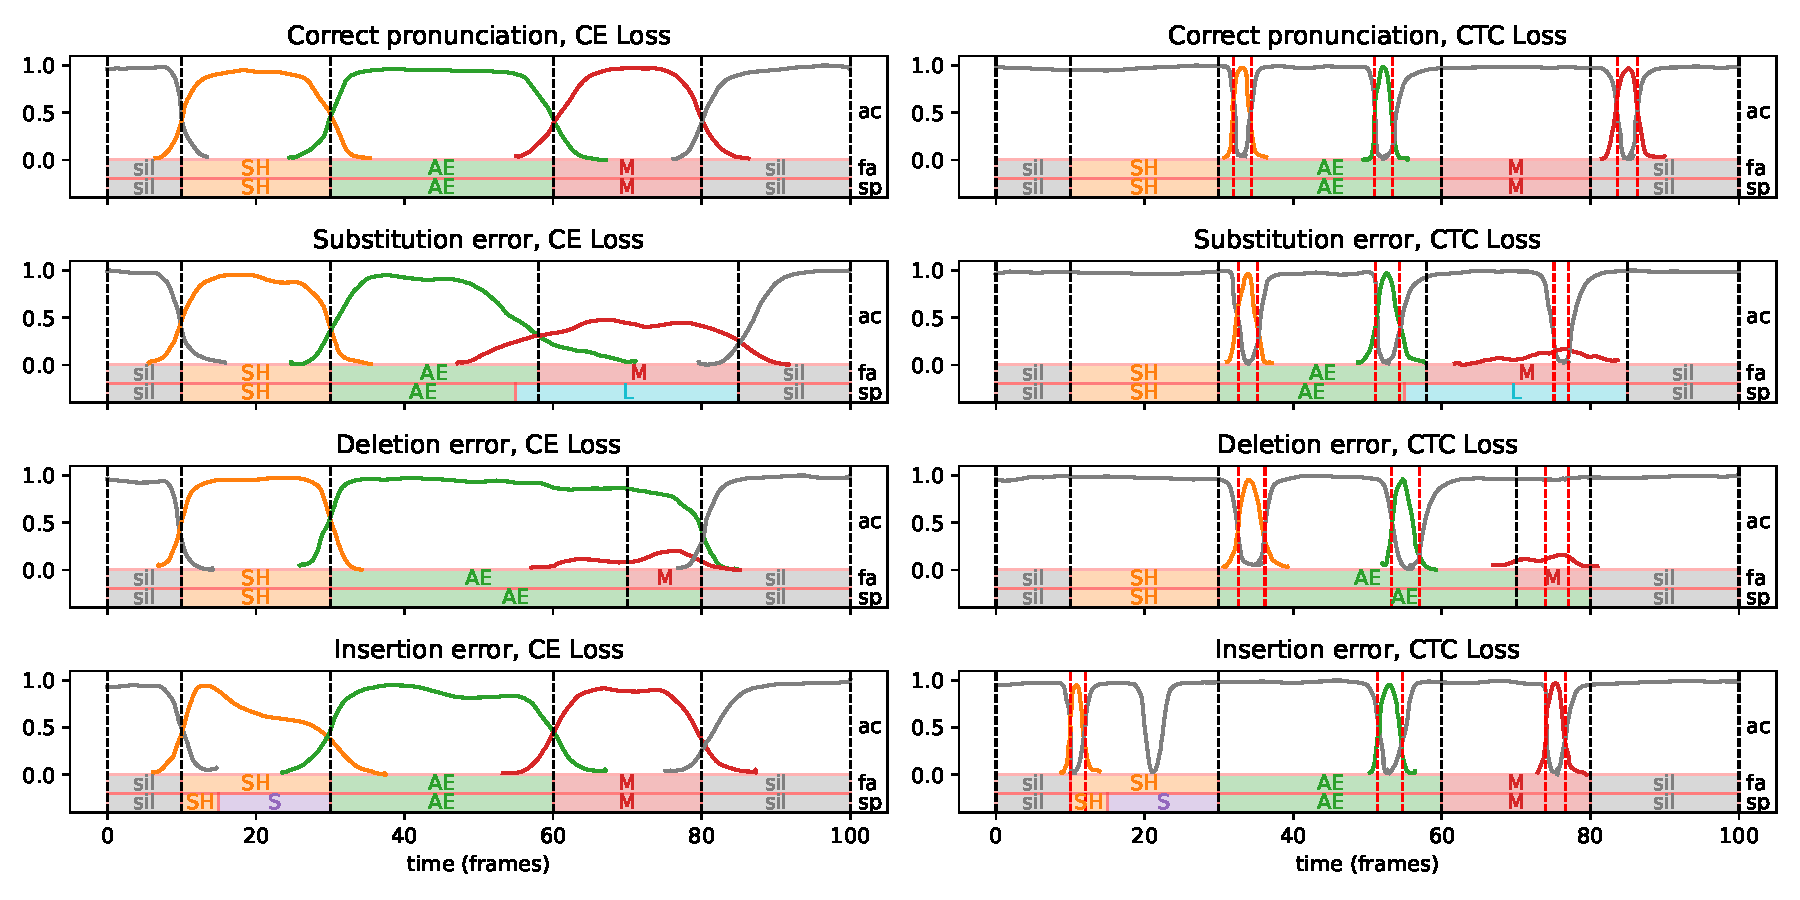
\includegraphics[width=\linewidth]{figs/method_illustration.pdf}
  \caption{Illustration of the issues with standard GOP methods for models trained with CE loss (left) and CTC loss (right). Each plot corresponds to a different kind of mispronunciation and is divided in three parts: ``sp'' shows that segments that were actually spoken; ``fa'' shows the forced alignment based on the canonical pronunciation; ``ac'' shows the activations from the model and for the canonical segments. Finally, for the CTC models, the red dashed lines show the alternative forced alignment from the GOP-CTC-align method. }
  %Simulated mispronunciation of the word ``sham'' can cause segmentation mismatch compared to the ground truth with the forced alignment based on CE-trained model~(left). However, for CTC-trained model~(right), the the segmentation for any canonical phoneme is less affected by the mispronunciation.}
  \label{fig:illustration-alignment-problems}
\end{figure*}  

\subsection{End-to-end ASR models, CTC and peaky behavior}
\label{sec:peaky_behavior}
%End-to-end ASR aims at simplifying the traditional ASR's workflow and reduce the requirement of domain knowledge as much as possible.
%The traditional ASR often comprises several components: the acoustic model, the language model, the phonetic dictionary etc.
%On the contrary, for End-to-end ASR, only a single but powerful DNN is trained to predict the transcription directly from input speech. 
In this section, we introduce some details of the Connectionist Temporal Classification (CTC) loss used in modern end-to-end ASR models.
This premise is important to understand our methods in Section~\ref{sec:Methods}.

End-to-end ASR models were initially introduced to map speech to output symbols, typically characters\footnote{The methods for MDD described in this paper use phonemes as output symbols. However, all the arguments in this section apply regardless of the nature of the output symbols.}, directly.
In general, the sequence of output symbols $L = \{l_1, \dots, l_{|L|}\}$ has a different rate that the input speech feature vectors $O_1^T = \{o_1, \dots, o_T\}$.
To overcome this problem in training, the CTC loss~\cite{CTC} was introduced.
This makes use of an additional blank ($\phi$) output symbol.
%CTC-based ASR systems are characterized by their additional blank ($\phi$) output symbol.
%We denote the vocabulary for CTC as $V$ which is the set of all legal symbols\footnote{For ASR, the output symbols are usually characters. Since we are discussing here MDD at phoneme-level throughout the paper, the CTC models are trained to output canonical phoneme sequences.} $C$ plus the special blank token: $ V = C \cup \{\phi\}$.
Given a speech sequence $O_1^T$ of length $T$, we define $V$ as the set of all output symbols including $\phi$.
Then any vector $u = \{u_1, \dots, u_T\} \in U = V^T$ is an alignment path between the input sequence and the output symbols.
The probability of a path $u$ under the assumption of conditional independence is $p(u| O_{1}^{T})=\prod_{t=1}^{T}p(u_t|o_t)$.
As a consequence $\sum_{u \in U}p(u| O_{1}^{T}) = 1$ representing all possible paths given the model and the speech.
During training, for a given target output sequence $L$ and the speech sequence $O_{1}^{T}$, the model learns to minimize the following loss:
% of the target sequence directly, without having to obtain frame-wise labels.
% Formally, the CTC loss function for $L_\text{target}$ is defined to be:
% \begin{equation}
% \label{eqa:CTC-loss} 
% \begin{aligned}
%    \pounds_{CTC} &= -\log{\mathit{p}(L_\text{target}|O_{1}^{T})}                
% \end{aligned}
% \end{equation} 
% The posterior probability of the target label sequence is the summation of the probability of all paths corresponding to the target: 
\begin{equation}
   \label{eqa:CTC-loss}
    \mathcal{L}_{\text{CTC}}(L) = -\log\sum_{\pi \in {\{u:\mathcal{B}(u) = L\}}} p(\pi|O_1^T) 
\end{equation}
where $\pi$ spans over the paths that can be mapped to $L$ using the many-to-one function: $\mathcal{B}: U \rightarrow L$ by removing all repeated symbols and followed by removal of the blank symbols, e.g., $\mathcal{B}(a{\phi}b{\phi}b{\phi}cc{\phi})$ $=$ $abbc$. 

Since training the CTC does not require frame-level alignment, the timing information tends to be ignored by the model.
A well-known phenomenon of CTC-trained model is the ``peaky'' behavior of model output, as illustrated in the right column of Figure~\ref{fig:illustration-alignment-problems}.
There are two dimensions of peakiness: ``peaky over time'' (POT) and ``peaky over state'' (POS).
%, as shown in the first row~(right) of Fig.~\ref{fig:illustration-alignment-problems}: 
POT behavior corresponds to the fact that the blank symbol is activated for most of the time steps, whilst the non-blank symbols that correspond to the target label sequence only become activated for a few time steps. 
Forced alignment (Viterbi search) performed with CTC-trained models can result in distorted alignment between input speech and output symbols.
On the other hand, POS behavior is observed because the model activations at each frame are always close to 1.0 for one output and 0.0 for all the others.
%POS is an indication of overfitting of model which represents a distribution of all paths but centered at one single instance---the Viterbi path. 
%This is not consistent with the observation of ambiguous alignment, as discussed in Section~\ref{sec:alignment_issues}.

For these reasons, CTC is not feasible for applications where the time alignment is essential, such as voice activity detection, speech segmentation, or conventional GOP evaluation for MDD.
An indication of this is the lack of literature in these areas that use CTC-based models.
%to many temporal-sensitive speech applications such as voice activity detection. 
%We believe that for the same reason, CTC is rarely connected with the conventional alignment-based GOP for MDD in the literature. 
However, several works tried to mitigate the peaky behavior of CTC-based models for ASR, e.g.~\cite{why_peaky, CTC-ME, huang2024peakyaccuratectcforced}.
% In~\cite{cao24b_interspeech}, the authors show that CTC-trained models can be used for GOP~(GOP-CTC-AF and GOP-CTC-Align) despite CTC's peaky behavior.
% In this work, we will further discuss the impact of peakiness for MDD using both traditional GOP (GOP-DNN-Avg) and the CTC-based GOP from~\cite{cao24b_interspeech}.

The two methods proposed in this paper, have as goal to make it possible to use CTC-trained models with phoneme output targets as a basis for computing GOP for MDD tasks.
%we will follow our previous work~\cite{cao24b_interspeech} and further discuss the rationale behind using CTC-trained model for GOP.

